\section{COMPSs Tools}
\label{sec:Tools}

%%%%%%%%%%%%%%%%%%%%%%%%%%%%%%%%%%%%%%%%%%%%%%%%%%%%%%%
%%%%%%%%%%%%%%%%% APPLICATION GRAPH %%%%%%%%%%%%%%%%%%%
%%%%%%%%%%%%%%%%%%%%%%%%%%%%%%%%%%%%%%%%%%%%%%%%%%%%%%%
\subsection{Application graph}
At the end of the application execution a dependency graph can be generated representing the order of execution of each type of 
task and their dependencies. To allow the final graph generation the runcompss command must be run with the \textit{-g} flag 
and the final graph will appear at the \textit{$base\_log\_folder$}$/monitor/complete\_graph$.dot at the end of the execution.

Figure \ref{fig:complete_graph} shows a dependency graph example of a \textit{SparseLU} java application. The graph can be
visualized by running the following command:
\begin{lstlisting}[language=bash]
compss@bsc:~$ gengraph ~/.COMPSs/sparseLU.arrays.SparseLU_01/monitor/complete_graph.dot
\end{lstlisting}

\begin{figure}[h!]
  \centering
    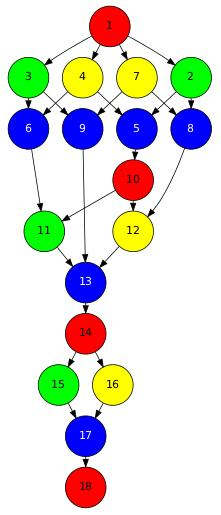
\includegraphics[width=0.3\textwidth]{./Sections/4_Tools/Figures/dependency_graph.jpeg}
    \caption{The dependency graph of the SparseLU application}
    \label{fig:complete_graph}
\end{figure}



%%%%%%%%%%%%%%%%%%%%%%%%%%%%%%%%%%%%%%%%%%%%%%%%%%%%%%%
%%%%%%%%%%%%%%%%%%%%%%%% MONITOR %%%%%%%%%%%%%%%%%%%%%%
%%%%%%%%%%%%%%%%%%%%%%%%%%%%%%%%%%%%%%%%%%%%%%%%%%%%%%%
\subsection{COMPSs Monitor}
\label{subsec:monitor}
The COMPSs Framework exposes a Web Service with a graphical interface that can be used to monitor either finished 
and running applications. COMPSs Monitor is installed as a service and can be easily managed by running any of the following
commands:
\begin{lstlisting}[language=bash]
compss@bsc:~$ sudo service compss-monitor usage
Usage: /usr/sbin/service compss-monitor 
           {start | stop | reload | restart | try-restart | force-reload | status}
\end{lstlisting}

\subsubsection{Service configuration}
The COMPSs Monitor service can be configured by editing the \textit{/opt/COMPSs/Tools/}
\textit{monitor/apache-tomcat/conf/compss-monitor.conf}
file which contains one line per property:
\begin{itemize}
 \item \textbf{$IT\_MONITOR$} Default directory to retrieve monitored applications.
 \item \textbf{$COMPSs\_MONITOR\_PORT$} Port where to run the compss-monitor web service.
 \item \textbf{$COMPSs\_MONITOR\_TIMEOUT$} Web page timeout between browser and server.
\end{itemize}

By default, the $IT\_MONITOR$ points to the \textit{.COMPSs} folder inside the \textit{root} user, opens the web service in the 
port 8080 and has a 20s timeout. 

\subsubsection{Usage}
In order to use the COMPSs Monitor users need to start the service as shown in Figure \ref{fig:monitor_start}.
\begin{figure}[thb!]
  \centering
    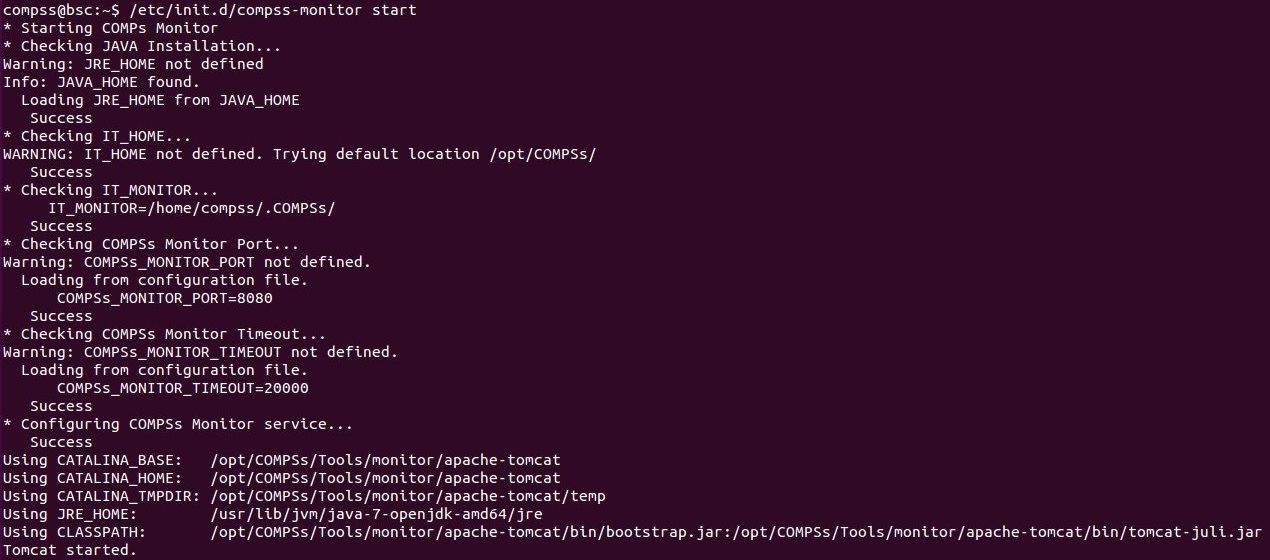
\includegraphics[width=\textwidth]{./Sections/4_Tools/Figures/monitor_start.jpeg}
    \caption{COMPSs Monitor start command}
    \label{fig:monitor_start}
\end{figure}

And use a web browser to open the specific URL:
\begin{lstlisting}[language=bash]
compss@bsc:~$ firefox http://localhost:8080/compss-monitor &
\end{lstlisting}

The COMPSs Monitor allows to monitor applications from different users and thus, users need to login first to grant access 
to their applications. Once done, as shown in Figure \ref{fig:monitoring_interface}, the users can select any of their executed
or on-going COMPSs applications and display it.
\begin{figure}[thb!]
  \centering
    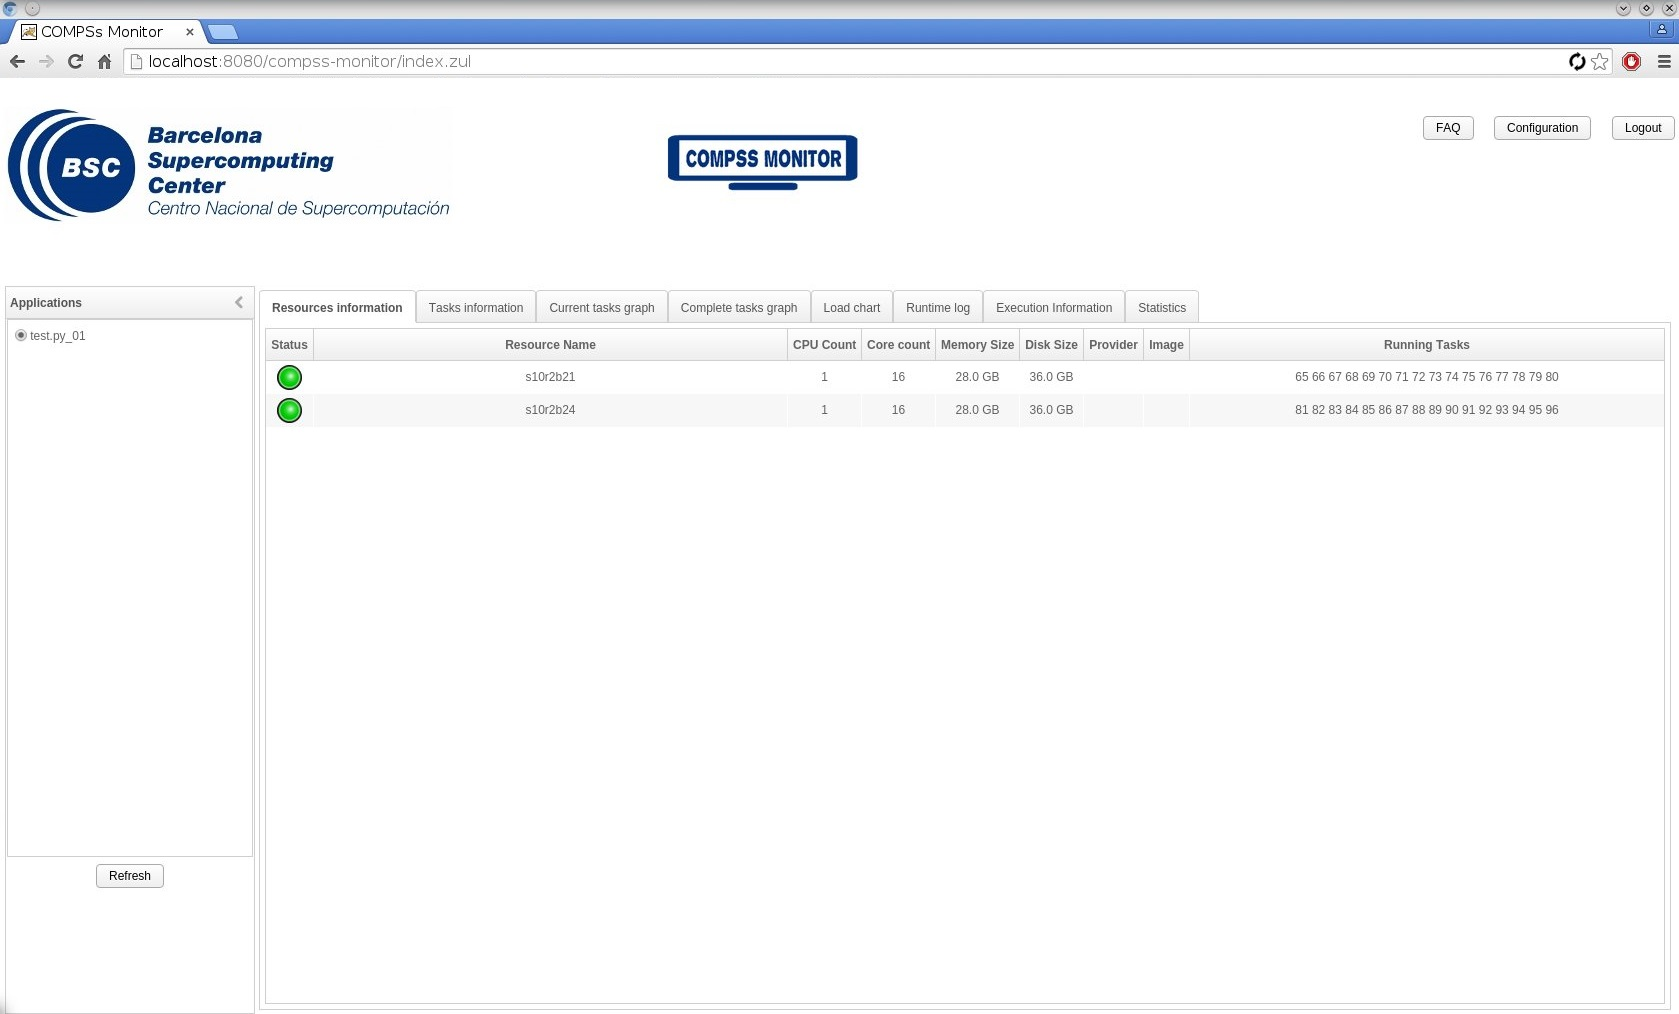
\includegraphics[width=0.95\textwidth]{./Sections/4_Tools/Figures/compss_monitor.jpeg}
    \caption{COMPSs monitoring interface}
    \label{fig:monitoring_interface}
\end{figure}

To enable \textbf{all} the COMPSs Monitor features, applications must run the runcompss command with the \textit{-m} flag. This flag 
allows the  COMPSs Runtime to store special information inside inside the \textit{log base folder} under the \textit{monitor} 
folder (see Figures \ref{fig:simple_exec_monitor} and \ref{fig:simple_logs_monitor}). Only advanced users should modify or delete any of these files. If the application that a user is trying to monitor 
has not been executed with this flag, some of the COMPSs Monitor features will be disabled. 
\begin{figure}[ht!]
  \centering
    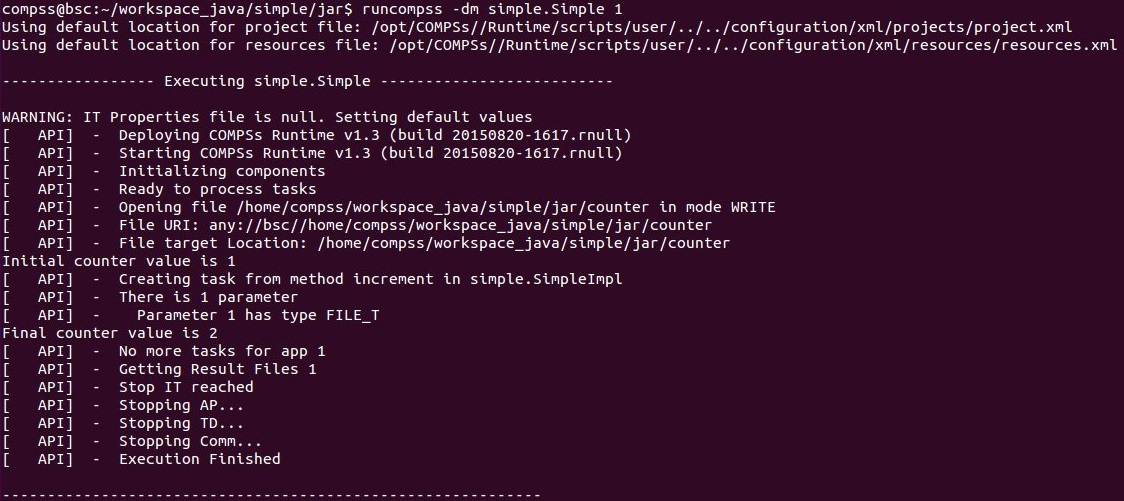
\includegraphics[width=0.95\textwidth]{./Sections/4_Tools/Figures/simple_monitor.jpeg}
    \caption{Execution of the Simple java application with the monitoring flag enabled}
    \label{fig:simple_exec_monitor}
\end{figure}

\begin{figure}[ht!]
  \centering
    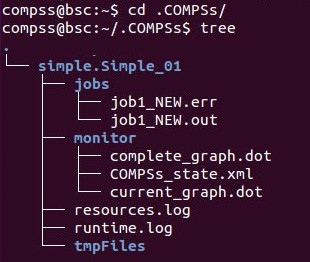
\includegraphics[width=0.4\textwidth]{./Sections/4_Tools/Figures/logs_with_monitor.jpeg}
    \caption{Logs generated by the Simple java application with the monitoring flag enabled}
    \label{fig:simple_logs_monitor}
\end{figure}

\newpage
\subsubsection{Graphical Interface features}
Next we provide a summary of the COMPSs Monitor supported features available through the graphical interface:
\begin{itemize}
 \item \textbf{Resources information} \newline
	Provides information about the resources used by the application
 \item \textbf{Tasks information} \newline
	Provides information about the tasks definition used by the application
 \item \textbf{Current tasks graph} \newline
	Shows the tasks dependency graph currently stored into the COMPSs Runtime
 \item \textbf{Complete tasks graph} \newline
	Shows the complete tasks dependecy graph of the application
 \item \textbf{Load chart} \newline
	Shows different dynamic charts representing the evolution over time of the resources load and the tasks load
 \item \textbf{Runtime log} \newline
	Shows the runtime log
 \item \textbf{Execution Information} \newline
	Shows specific job information allowing users to easily select failed or uncompleted jobs
 \item \textbf{Statistics} \newline
	Shows application statistics such as the accumulated cloud cost. 
\end{itemize}

\colorComment{\textbf{Attention}: To enable all the COMPSs Monitor features applications must run with the \textit{$-m$} flag.}

The webpage also allows users to configure some performance parameters of the monitoring service by accessing the 
\textit{Configuration} button at the top-right corner of the web page. 

For specific COMPSs Monitor feature configuration please check our \textit{FAQ} section at the top-right corner of the web page. 


%%%%%%%%%%%%%%%%%%%%%%%%%%%%%%%%%%%%%%%%%%%%%%%%%%%%%%%
%%%%%%%%%%%%%%%% APPLICATION TRACING %%%%%%%%%%%%%%%%%%
%%%%%%%%%%%%%%%%%%%%%%%%%%%%%%%%%%%%%%%%%%%%%%%%%%%%%%%
\subsection{Application tracing}
\label{sec:Tracing}
COMPSs Runtime can generate a post-execution trace of the distributed execution of the application. This trace is useful for
performance analysis and diagnosis.

A trace file may contain different events to determine the COMPSs master state, the task execution state or the file-transfers.
Despite the fact that in the current release we do not support file-transfers, we intend to support them in a near future release.

During the execution of the application, an XML file is created at worker nodes to keep track of 
these events. At the end of the execution, all the XML files are merged to get a final trace file.

In the following sections we explain the command used for tracing, how the events are registered, 
in a process called instrumentation, how to visualize the trace file and make a good analysis of 
performance based on the data shown in the trace.

\subsubsection{Trace Command}
In order to obtain a post-execution trace file the option \textbf{-t}  must be added to the runcompss command. Next we provide an
example of the command execution with the tracing option enabled for the Hmmer java application.
\begin{lstlisting}[language=bash]
compss@bsc:~$ runcompss -t --classpath=/home/compss/workspace_java/hmmerobj/jar/hmmerobj.jar 
                        hmmerobj.HMMPfam 
                        /sharedDisk/Hmmer/smart.HMMs.bin /sharedDisk/Hmmer/256seq 
                        /home/compss/out.txt 2 8 -A 222
\end{lstlisting}
 

\subsubsection{Application Instrumentation}
The instrumentation is the process that intercepts different events of the application execution 
and keeps log of them. This will cause an overhead in the execution time of the application that 
the user should take into account, but the collected data will be extremely useful for performance 
analysis and diagnosis.

COMPSs Runtime uses the \textit{Extrae} tool to dynamically instrument the application and the \textit{Paraver} tool to visualize
the obtained tracefiles. Both tools are developped at \textit{BSC} and are available in its webpage \url{http://bsc.es} . 

At the worker nodes, in background, \textit{Extrae} keeps track of the events in an intermediate format 
file (with \textit{.mpit} extension). Inside the master node, at the end of the execution, \textit{Extrae} merges the 
intermediate files to get the final trace file, a \textit{Paraver} format file (.prv). See the visualization 
section \ref{subsubsec:paraver} in this manual for further information about the \textit{Paraver} tool.

When instrumenting the application \textit{Extrae} will output several messages. At the master node, \textit{Extrae} will show up its
initialization at the begining of the execution and the merging process and the paraver generation at the end of the execution. At the
worker nodes \textit{Extrae} will inform about the intermediate files generation every time a task is executed. Next we provide a 
summary of the \textit{stdout} generated by Hmmer java application execution with the trace flag enabled. 
\begin{lstlisting}[language=bash]
----------------- Executing hmmerobj.HMMPfam --------------------------

WARNING: IT Properties file is null. Setting default values
Welcome to Extrae 3.1.1rc (revision 3360 based on extrae/trunk)
Extrae: Warning! EXTRAE_HOME has not been defined!.
Extrae: Generating intermediate files for Paraver traces.
Extrae: Intermediate files will be stored in /home/compss/workspace_java/hmmerobj/jar
Extrae: Tracing buffer can hold 500000 events
Extrae: Tracing mode is set to: Detail.
Extrae: Successfully initiated with 1 tasks

Extrae: Warning! API tries to initialize more than once
Extrae:          Previous initialization was done by API

[   API]  -  Starting COMPSs Runtime v1.3 (build 20150821-1134.rnull)

...
...
...

[   API]  -  No more tasks for app 1
[   API]  -  Getting Result Files 1
[   API]  -  Execution Finished

Extrae: Intermediate raw trace file created : /home/compss/workspace_java/hmmerobj/jar/set-0/TRACE@bsc.0000031637000000000000.mpit
Extrae: Intermediate raw sym file created : /home/compss/workspace_java/hmmerobj/jar/set-0/TRACE@bsc.0000031637000000000000.sym
Extrae: Deallocating memory.
Extrae: Application has ended. Tracing has been terminated.

merger: Output trace format is: Paraver
merger: Extrae 3.1.1rc (revision 3360 based on extrae/trunk)

mpi2prv: Checking for target directory existance... exists, ok!
mpi2prv: Selected output trace format is Paraver
mpi2prv: Stored trace format is Paraver
mpi2prv: Parsing intermediate files
mpi2prv: Removing temporal files... done
mpi2prv: Congratulations! ./trace/hmmerobj.HMMPfam_compss_trace_1440151114.prv has been generated.

------------------------------------------------------------
\end{lstlisting}

For further information about \textit{Extrae} please visit the following site: 
\begin{center}
\url{http://www.bsc.es/computer-science/extrae} 
\end{center}


\subsubsection{Trace Visualization}
\label{subsubsec:paraver}
\textit{Paraver} is the \textit{BSC} tool for trace visualization. Trace events are encoded in \textit{Paraver} format (\textit{.prv}) 
by the \textit{Extrae} tool (see previous section). \textit{Paraver} is a powerful tool that allows users to show many 
views of the trace data by means of different configuration files. Users can manually load, edit or create configuration files to
obtain different trace data views. 

In the following subsections we will explain how to load a trace file into \textit{Paraver}, open the task 
events view by means of an already predefined configuration file, and how to 
adjust the view to properly display the data.

For further information about \textit{Paraver} please visit the following site:
\begin{center}
\url{http://www.bsc.es/computer-sciences/performance-tools/paraver}
\end{center}

\paragraph{Trace Loading}
The final trace file in \textit{Paraver} format (.\textit{prv}) can be found at the \textit{base log folder} of the application
execution inside the trace folder. The fastest way to open it is calling directly the \textit{Paraver} binary using the trace-file name
as arugment.
\begin{lstlisting}[language=bash]
compss@bsc:~$ wxparaver /home/compss/.COMPSs/hmmerobj.HMMPfam_01/trace/*.prv
\end{lstlisting}
 
\paragraph{Configuration File}
In order to open a view with the task events of the application, an already predefined configuration 
file is provided. To open it, just go in the main window to the ``Load Configuration'' option in 
the menu ``File''. The configuration file is under the following path \textit{/opt/COMPSs/Dependencies/paraver/cfgs/tasks.cfg}. 
After accepting the load of the configuration file, another window will appear to show the view. Figures \ref{fig:trace_1} and
\ref{fig:trace_2} show an example of this process.

\begin{figure}[ht!]
  \centering
    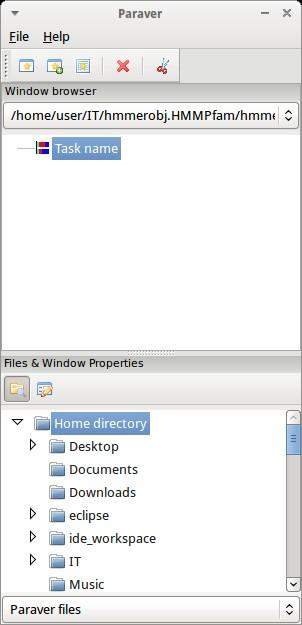
\includegraphics[width=0.45\textwidth]{./Sections/4_Tools/Figures/1.jpeg}
    \caption{Paraver menu}
    \label{fig:trace_1}
\end{figure}

\begin{figure}[ht!]
  \centering
    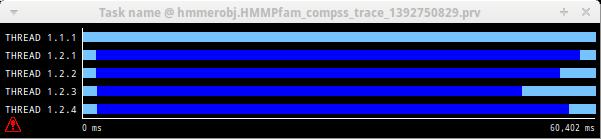
\includegraphics[width=1.0\textwidth]{./Sections/4_Tools/Figures/2.jpeg}
    \caption{Trace file}
    \label{fig:trace_2}
\end{figure}

\paragraph{View Adjustment}
In a \textit{Paraver} view, a red exclamation sign may appear on the bottom-left corner (see last Figure \ref{fig:trace_2} in 
previous section). This means that some little adjustments must be done to view the trace correctly:

\begin{itemize}
 \item Fit window: this will give a better color scale to identify events.
	\begin{itemize}
	    \item Right click on the trace window
	    \item Chose the option Fit Semantic Scale / Fit Both
	\end{itemize}
\end{itemize}

\begin{figure}[ht!]
  \centering
    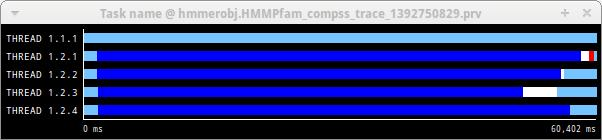
\includegraphics[width=1.0\textwidth]{./Sections/4_Tools/Figures/3.jpeg}
    \caption{Paraver view adjustment: Fit window}
\end{figure}

\begin{itemize} 
 \item View Event Flags: This will put a flag whenever an event starts/ends.
	\begin{itemize}
	    \item Right click on the trace window
	    \item Chose the option View / Event Flags
	\end{itemize}
\end{itemize}
 
\begin{figure}[ht!]
  \centering
    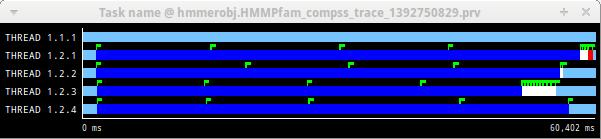
\includegraphics[width=1.0\textwidth]{./Sections/4_Tools/Figures/4.jpeg}
    \caption{Paraver view adjustment: View Event Flags}
\end{figure}

\begin{itemize}
 \item Show Info Panel: This will show an information panel. In the tab ``Colors'' we can see the legend of the colors shown in the view.
	\begin{itemize}
	    \item Right click on the trace window
	    \item Check the Info Panel option
	    \item Select the Colors tab in the panel
	\end{itemize}
\end{itemize}

\begin{figure}[ht!]
  \centering
    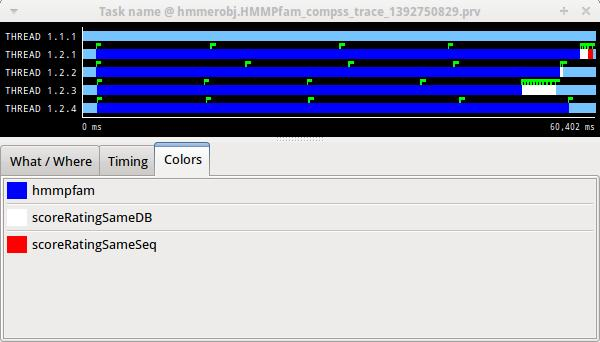
\includegraphics[width=1.0\textwidth]{./Sections/4_Tools/Figures/5.jpeg}
    \caption{Paraver view adjustment: Show info panel}
\end{figure}

\begin{itemize}
 \item Zoom: In order to understand a trace view better, sometimes it’s a worth thing to zoom into it a little.
	\begin{itemize}
	    \item Select a region in the trace window to see that region in detail
	    \item And repeat the previous step as many times as needed
	    \item The undo-zoom option is in the right click panel
	\end{itemize}
\end{itemize}

\begin{figure}[ht!]
  \centering
    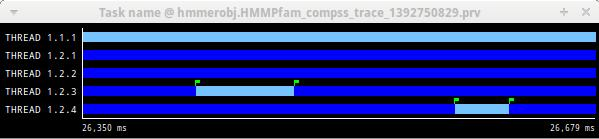
\includegraphics[width=1.0\textwidth]{./Sections/4_Tools/Figures/6.jpeg}
    \caption{Paraver view adjustment: Zoom configuration}
\end{figure}

\begin{figure}[ht!]
  \centering
    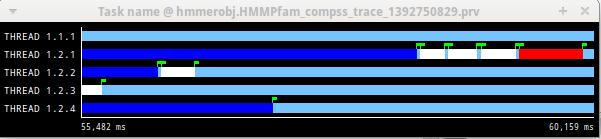
\includegraphics[width=1.0\textwidth]{./Sections/4_Tools/Figures/6_2.jpeg}
    \caption{Paraver view adjustment: Zoom configuration}
\end{figure}


\subsubsection{Trace Interpretation}
In this section we will explain how to interpret a trace view once it has been adjusted as 
described in the previous section.

\begin{itemize}
 \item The trace view has in its horizontal axis the execution time and in the vertical 
       axis one line for the master at the top, and below it, one line for each of the workers.
 \item In a line, the light blue color means idle state, in the sense that there is no event at that time.
 \item Whenever an event starts or ends a flag is shown.
 \item In the middle of an event, the line shows a different color. Colors are assigned depending on the event type.
 \item In the info panel the legend of assigned color to event type is provided.
\end{itemize}

\begin{figure}[ht!]
  \centering
    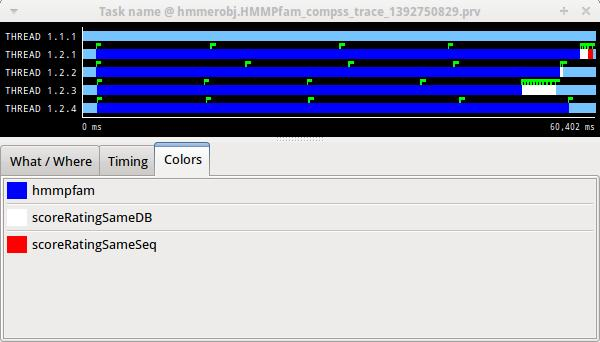
\includegraphics[width=\textwidth]{./Sections/4_Tools/Figures/7.jpeg}
    \caption{Trace interpretation}
\end{figure}


\subsubsection{Trace Analysis}
In this section, we will give some tips to analyse a COMPSs trace from two different points of view:
graphically and numerically.

\paragraph{Graphical Analysis}
The main concept is that computational events, the task events in this case, must be well 
distributed among all workers to have a good parallelism, and the duration of task events 
should be also balanced, this means, the duration of computational bursts.

\begin{figure}[ht!]
  \centering
    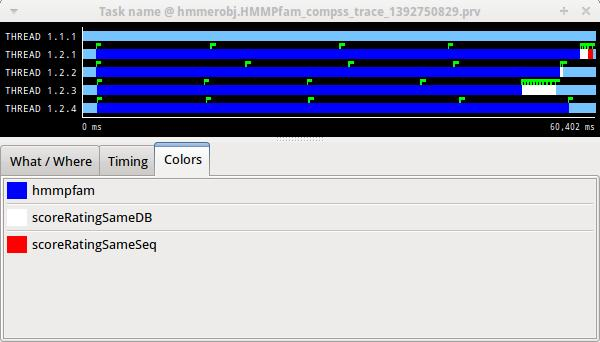
\includegraphics[width=1.0\textwidth]{./Sections/4_Tools/Figures/8.jpeg}
    \caption{Caption.}
\end{figure}

In the previous trace view, all the tasks of type ``hmmpfam'' in dark blue appear to be well 
distributed among the four workers, each worker executes four ``hmmpfam'' tasks.

But some workers finish earlier than the others, worker 1.2.3 finish the first and worker 1.2.1 
the last. So there is an imbalance in the duration of ``hmmpfam'' tasks. The programmer should 
analyse then whether all the tasks process the same amount of input data and do the same thing 
in order to find out the reason of such imbalance.

Another thing to highlight is that tasks of type ``scoreRatingSameDB'' are not equal distributed 
among all the workers. There are workers that execute more tasks of this type than the others. 
To understand better what happens here, let’s take a look to the execution graph and also zoom 
in the last part of the trace.

\begin{figure}[ht!]
  \centering
    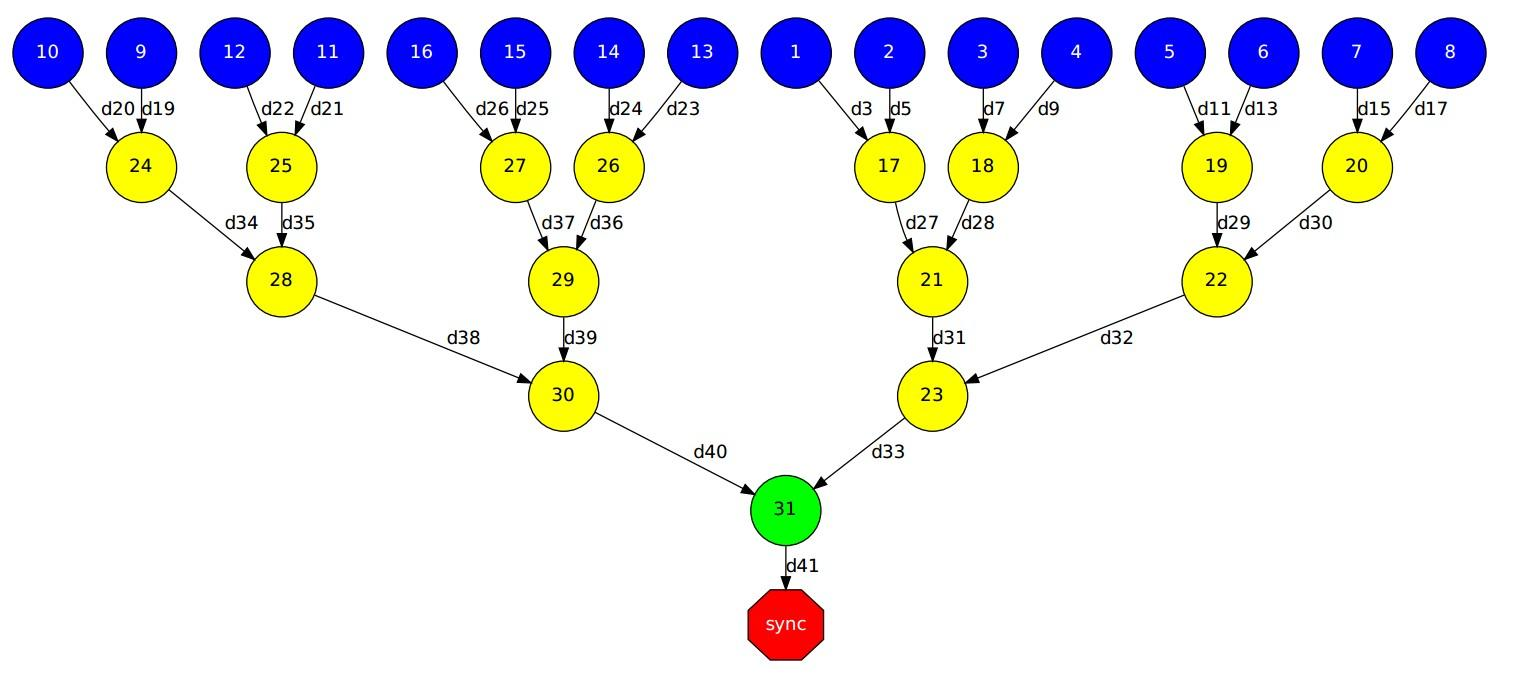
\includegraphics[width=1.0\textwidth]{./Sections/4_Tools/Figures/9.jpeg}
    \caption{Caption.}
\end{figure}

\begin{figure}[ht!]
  \centering
    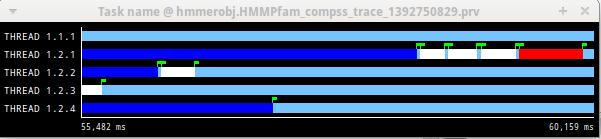
\includegraphics[width=1.0\textwidth]{./Sections/4_Tools/Figures/10.jpeg}
    \caption{Caption.}
\end{figure}

There is only one task of type ``scoreRatingSameSeq''. This task appears in red in the trace 
(and in light-green in the graph). With the help of the graph we see that the ``scoreRatingSameSeq'' 
task has dependences on tasks of type ``scoreRatingSameDB'', in white (or yellow).

When the last task of type ``hmmpfam'' (in dark blue) ends, the last dependences are solved, 
and if we look at the graph, this means going across a path of three dependences of type 
``scoreRatingSameDB'' (in yellow). And because of these are sequential dependences (one depends 
on the previous) no more than a worker can be used at the same time to execute the tasks. 
This is the reason of why the last three task of type ``scoreRatingSameDB'' (in white) are 
executed in worker 1.2.1 sequentially.

\paragraph{Numerical Analysis}
Here we show another trace from a different parallel execution of the Hmmer program.
 
\begin{figure}[ht!]
  \centering
    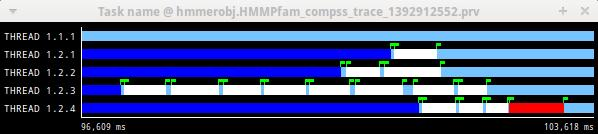
\includegraphics[width=1.0\textwidth]{./Sections/4_Tools/Figures/11.jpeg}
    \caption{Caption.}
\end{figure} 
 
Paraver offers the possibility of having different histograms of the trace events. 
For it just click the ``New Histogram'' button in the main window and accept the 
default options in the ``New Histogram'' window that will appear.

\begin{figure}[ht!]
  \centering
    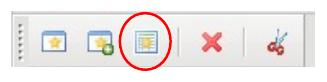
\includegraphics[width=0.5\textwidth]{./Sections/4_Tools/Figures/12.jpeg}
    \caption{Paraver Menu - New Histogram}
\end{figure}

After that, the following table is shown. In this case for each worker, the time spent 
executing each type of task is shown. Task names appear in the same color than in the 
trace view. The color of a cell in a row corresponding to a worker goes in a scale from 
a light-green for lower values to a dark-blue for higher ones. This conforms a color based histogram.

\begin{figure}[ht!]
  \centering
    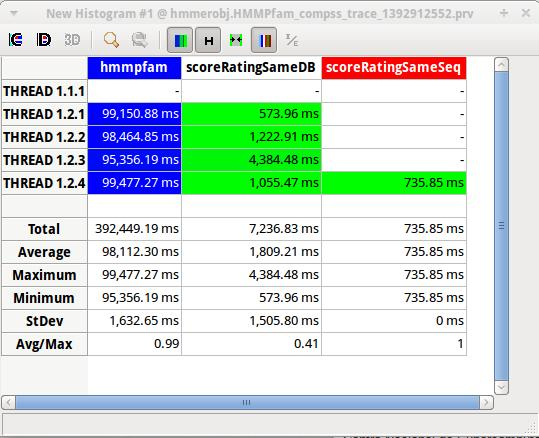
\includegraphics[width=0.8\textwidth]{./Sections/4_Tools/Figures/13.jpeg}
    \caption{Hmmpfam histogram}
\end{figure}
 
The previous table also gives, at the end of each column, some extra statistical 
information for each type of tasks (as the total, average, maximum or minimum values, etc.).

\newpage
In the window properties of the main window we can change the semantic of the statistics 
to see other factors rather than the time, for example, the number of bursts.

\begin{figure}[ht!]
  \centering
    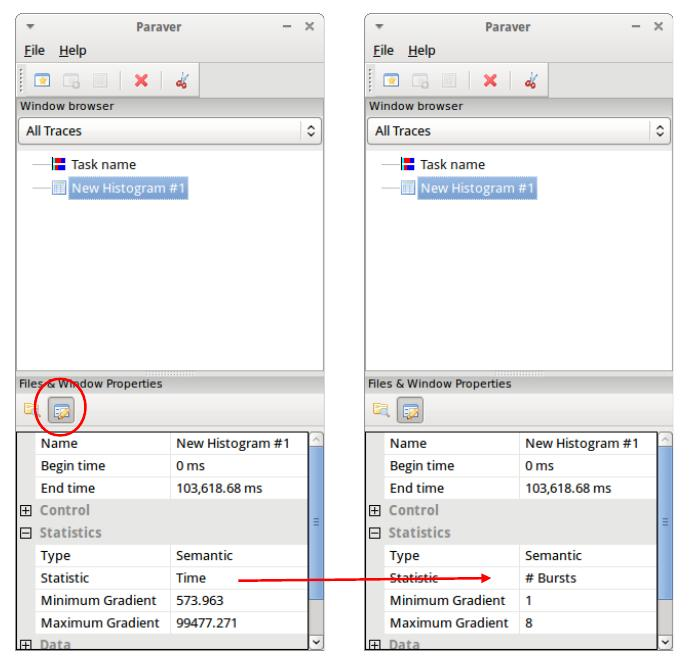
\includegraphics[width=0.8\textwidth]{./Sections/4_Tools/Figures/14.jpeg}
    \caption{Paraver histogram options menu}
\end{figure}

\newpage
In the same way as before, the following table shows for each worker the number of bursts 
for each type of task, this is, the number or tasks executed of each type. Notice the gradient 
scale from light-green to dark-blue changes with the new values.

\begin{figure}[ht!]
  \centering
    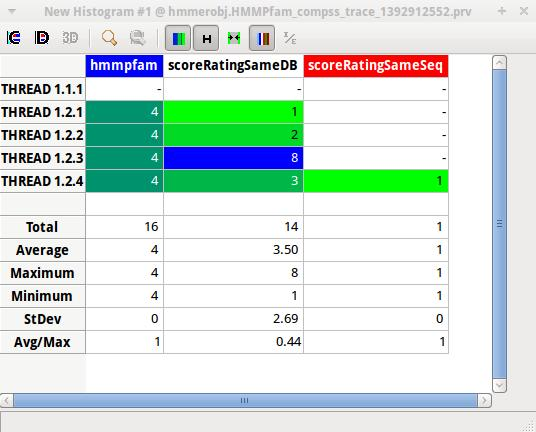
\includegraphics[width=0.8\textwidth]{./Sections/4_Tools/Figures/15.jpeg}
    \caption{Hmmpfam histogram with the number of bursts}
\end{figure}

\subsubsection{Other Trace examples}
To end this section, let’s present some other examples of COMPSs traces. COMPSs traces can be 
much complex as the number of workers or tasks grows. Just to illustrate this, the following 
pictures show traces with a greater number of workers and tasks.

\begin{figure}[ht!]
  \centering
    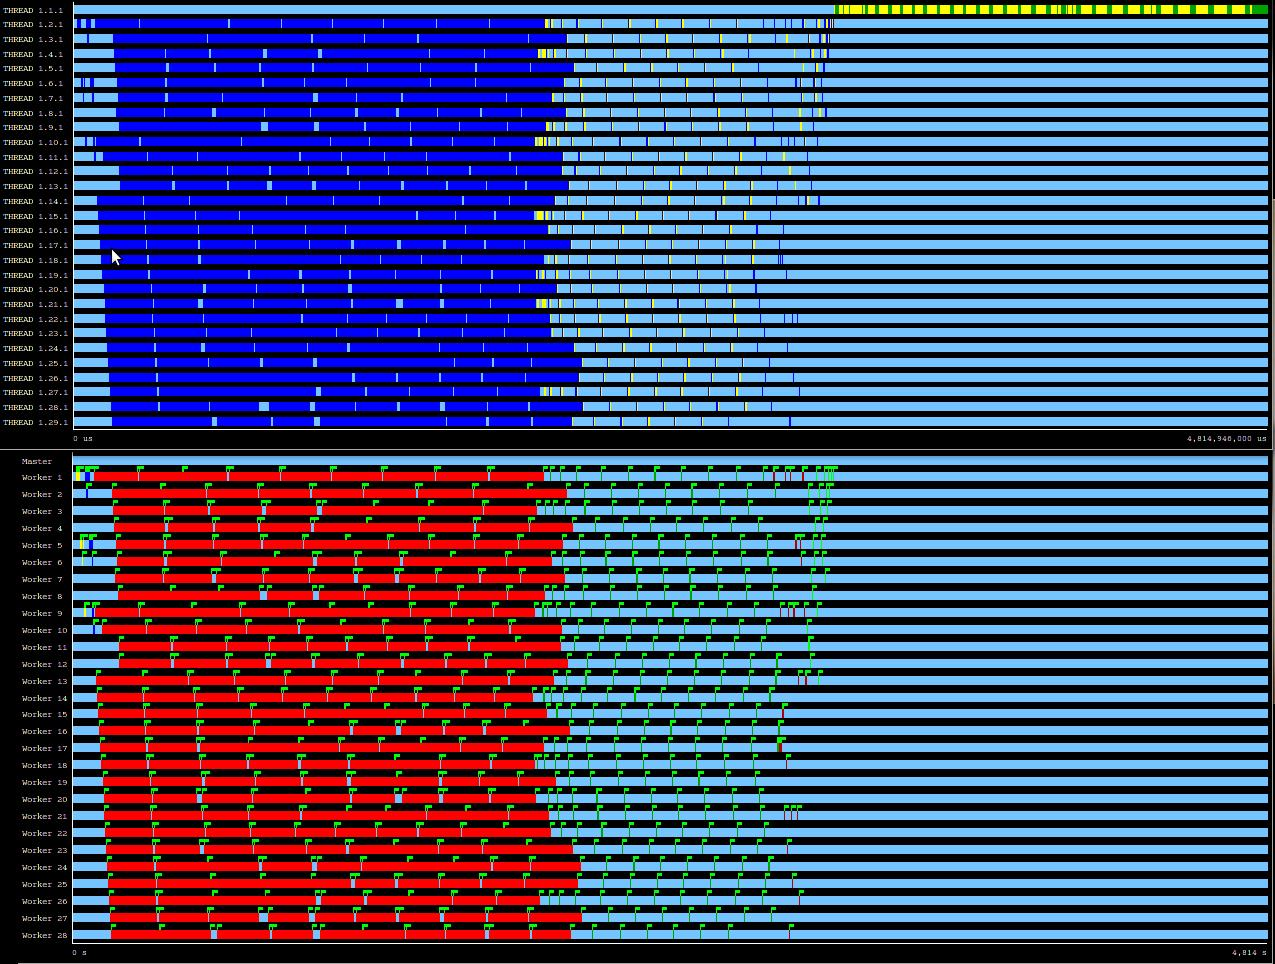
\includegraphics[width=0.91\textwidth]{./Sections/4_Tools/Figures/16.jpeg}
    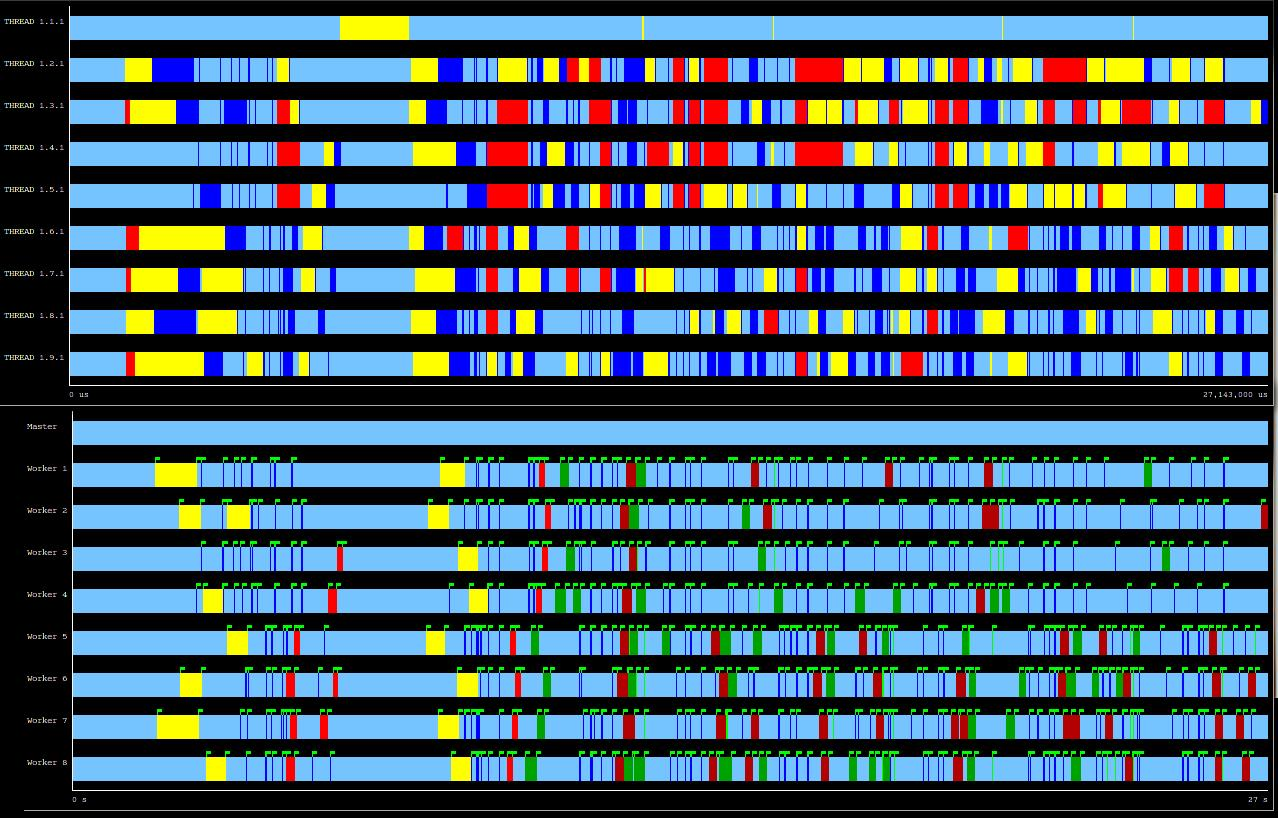
\includegraphics[width=0.91\textwidth]{./Sections/4_Tools/Figures/16_2.jpeg}
    \caption{Examples of complex traces}
\end{figure}

\newpage
%%%%%%%%%%%%%%%%%%%%%%%%%%%%%%%%%%%%%%%%%%%%%%%%%%%%%%%
%%%%%%%%%%%%%%%%%%%%%%%%% IDE %%%%%%%%%%%%%%%%%%%%%%%%%
%%%%%%%%%%%%%%%%%%%%%%%%%%%%%%%%%%%%%%%%%%%%%%%%%%%%%%%
\subsection{IDE}
\label{subsec:IDE}
The Eclipse IDE is available through the \textit{Eclipse Market}.